% 2015 江苏卷 第18题 题图：单圆锥曲线与少量直线
% 椭圆 x^2/2 + y^2 = 1，左准线 l: x = -2，右焦点 F(1,0)
% 过 F 的弦 AB（取代表性斜率 k=4），AB 的垂直平分线交 l、AB 于 P、C
\usetikzlibrary{arrows.meta}
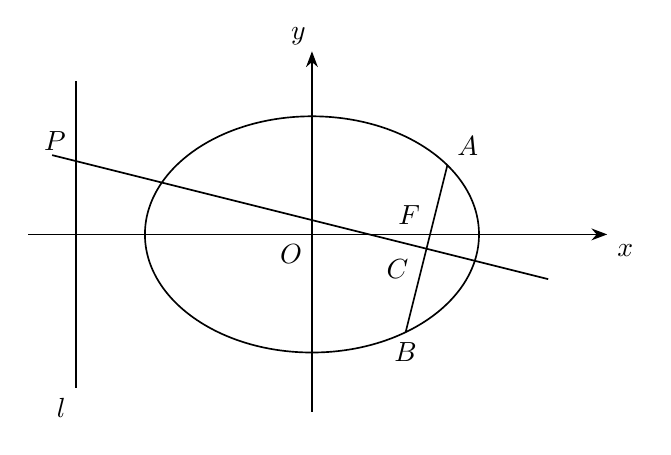
\begin{tikzpicture}[x=1.5cm,y=1.5cm,line width=.6pt,font=\normalsize,>=Stealth]
\def\ellA{1.41421356}
\def\ellB{1.00000000}
\coordinate (O) at (0.00000000,0.00000000);
\coordinate (F) at (1.00000000,0.00000000);
\coordinate (A) at (1.14639248,0.58556993);
\coordinate (B) at (0.79300146,-0.82799417);
\coordinate (C) at (0.96969697,-0.12121212);
\coordinate (P) at (-2.00000000,0.62121212);
\coordinate (Lbot) at (-2.00000000,-1.30000000);
\coordinate (Ltop) at (-2.00000000,1.30000000);
\coordinate (PB1) at (-2.20000000,0.67121212);
\coordinate (PB2) at (2.00000000,-0.37878788);
\draw[->] (-2.40000000,0.00000000)--(2.50000000,0.00000000) node[below right] {$x$};
\draw[->] (0.00000000,-1.50000000)--(0.00000000,1.55000000) node[anchor=south east,inner sep=0pt,xshift=-2pt,yshift=2pt] {$y$};
\draw (O) ellipse ({\ellA} and {\ellB});
\draw (Lbot)--(Ltop);
\draw (A)--(B);
\draw (PB1)--(PB2);
\node[below left] at (O) {$O$};
\node[above left] at (F) {$F$};
\node[above right] at (A) {$A$};
\node[below] at (B) {$B$};
\node at (0.72400000,-0.29340000) {$C$};
\node[above left] at (P) {$P$};
\node[below left] at (Lbot) {$l$};
\end{tikzpicture}
